\begin{event}{Sage Days 102, University of Ibadan}{SD102}{Ibadan (Nigeria), July 15 -- July 19, 2019}{PS}{80}{1}{https://opendreamkit.org/2019/07/29/SageDays102/}

\textbf{Main goals.} The purpose of this event was to introduce students,
lecturers, and reaserchers local to Nigeria, and some of the
neighboring countries, to \ODK software, particularly \Sage and \GAP,
as well as to improve their programming skills in general and foster
interest in contributing to open source mathematics software.

\textbf{\ODK implication.} Much of the initial animation for the event was
animated by Viviane Pons, though the only \ODK member to attend was
Erik Madison Bray, whose travel was funded by the project.  \ODK also
funded travel for three other instructors from outside the project, as
well as two PhD students who attended from neighboring countries
outside Nigeria.  All on-site facilities and logistics were funded by the
University of Ibadan.

\textbf{Event summary.} Significant time was spent helpint people install such
software on their personal machines: A particular challenge in Nigeria
where, as many attendees lacked reliable internet connections, even
downloading the software could pose a challenge.  The workshop was
primarily organized as a series of introductory lectures, including on
using the UNIX shell and basic Python programming, then moving on to
more application-specific uses of \Sage.  This included
topic-specific break-out sessions on numerical analysis, graph
theory, and algebraic combinatorics.  There were also successful
break-out sessions on group theory and abstract algebra with \GAP, and
statistical analysis with R. Participants also gave short talks on some
of their personal research and computational problems, and
participated in a contest to design interactive widgets for the Jupyter
notebook.

This workshop was a result of the Free Computational Mathematics conference at
CIRM earlier the same year, which had three visitors from the University
of Ibadan Department of Mathematics, and wanted to repeat the success of
that workshop at their home institution.


\textbf{Demographics.} Out of approximately 80 participants, most came from the
University of Ibadan as well as a few other institutions in Nigeria,
mostly in the southern and south-eastern regions of the country.  Two
students came from Ghana, as well as one from Congo.  One instructor
(originally from the United States) came from France, one (originally
from Ghana) came from Austria, and one (originally from Benin) came
from South Africa.  About one third of the attendees were women, and
there was a roughly equal mix of PhD students, postdocs, graduate
students, and a smaller number of professors an undergraduate students.

\textbf{Results and impact.} A full report on the impact of this
workshop can be read on our website:
\centerline{\url{https://opendreamkit.org/2019/07/29/SageDays102/}}

As there are relatiely few opportunities for many students in Nigeria to travel
outside the country, as there are few opportunities to meet with
outside lecturers, it's difficult to meet the demand for such
opportunities. Thus one of the primary goals of this workshop was to
disseminate the software itself, and to give a strong-enough
introduction to it that attendees could in turn introduce their peers
who were not able to attend, and to feel tapped into a broader
international community of researchers interested in computational
mathematics. To that end I believe we were successful, with 80\% of
attendees rating their knowledge of \Sage at 1 out of 5 before the
workshop, and over 90\% rating their knowelde at 3 or more after the
workshop.  83\% of attendees also felt highly confident that they had
been given the resources to continue to learning on their own, and to
find help with \Sage in the future, as well as that the workshop was
helpful for them to build opportunities for collaboration with their
peers.

Also, recognizing that one workshop was not enough to reach the demand for such
training, a group of the attendees spent the week incorporating an
organization (the strategy of which is still being developed) to build
local sustainability for this kind of training in the future, without
relying as much on (unfortunately rare) external support like that provided
by \ODK.


\begin{figure}[ht]
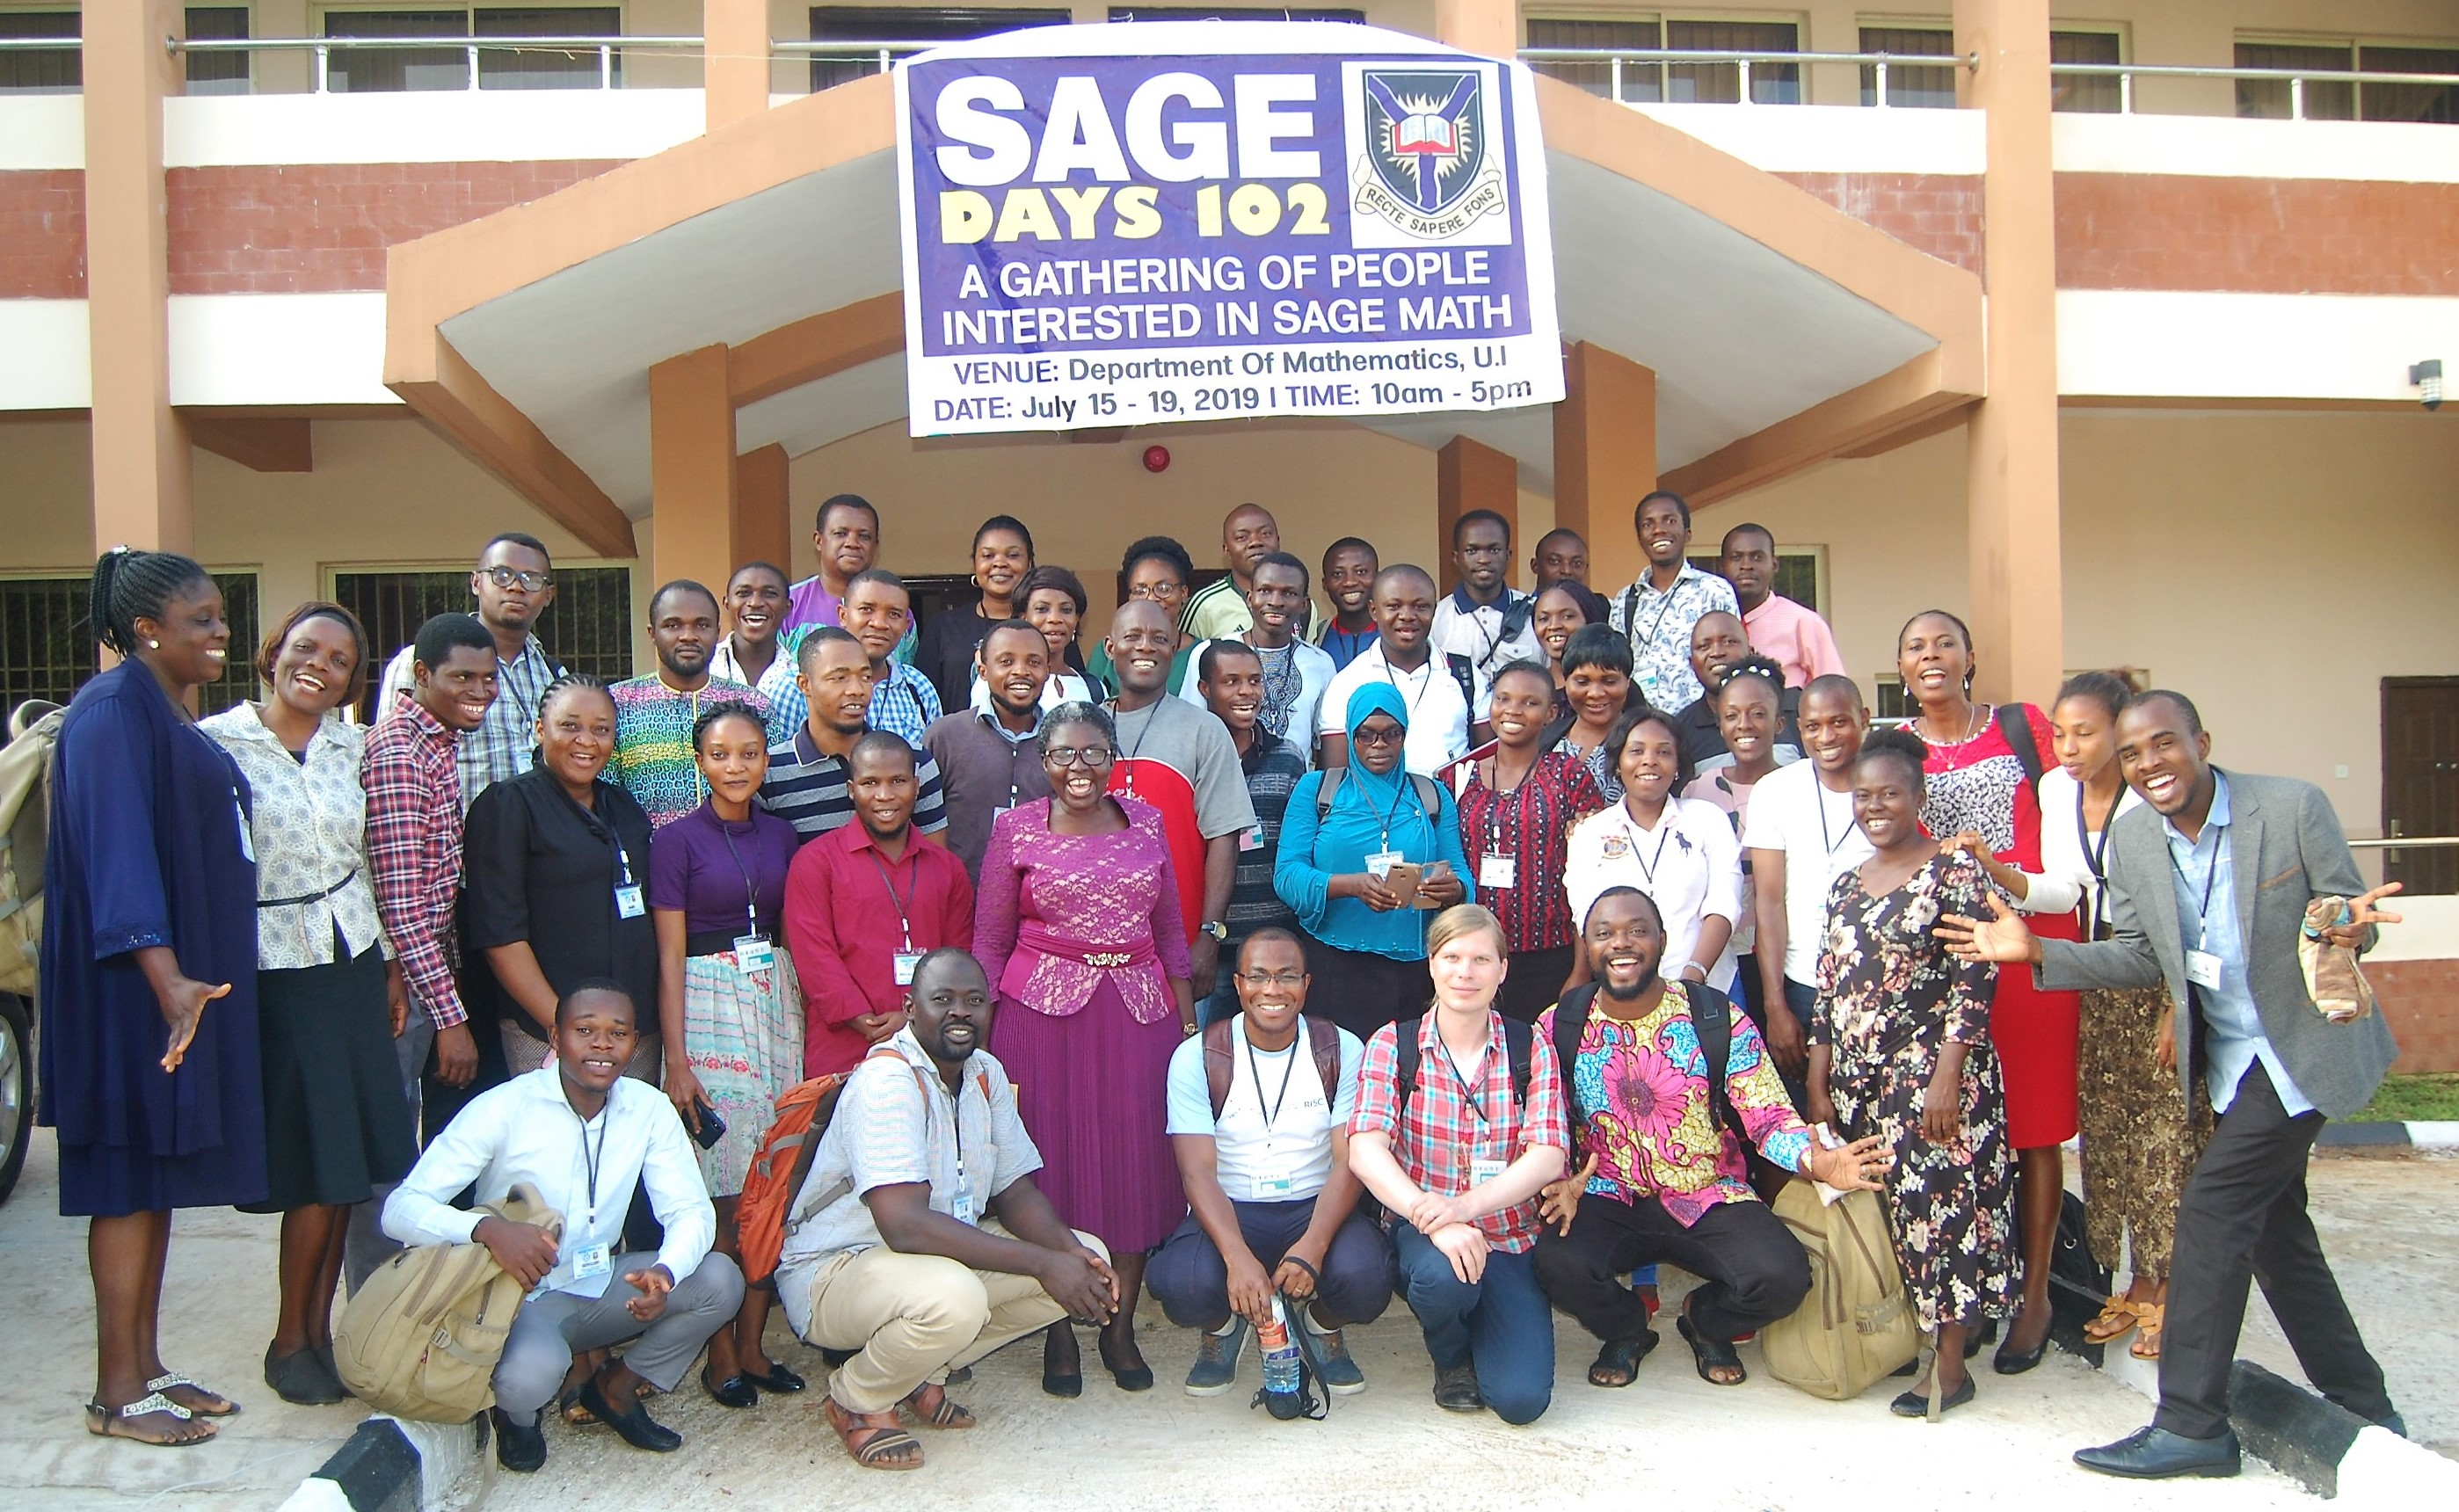
\includegraphics[scale=.5]{days102_group.jpg}
\caption*{Sage Days 102, University of Ibadan}
\end{figure}



\end{event}
